In section \ref{sec:cav_eom} we presented an amplitude field analysis of the canonical optomechanical system. The scope of this chapter is to apply the model to, in our case, a more appropriate system, i.e. the    membrane-in-the-middle, and see how the medium inside the cavity changes the cavity resonance as a function of membrane position $x$. We follow the approach presented in \cite{jayich2008, Wilson2011}. Our amplitude fields of the system are presented to the right in figure \ref{fig:transfer_model}.

\begin{figure}[H]
\centering
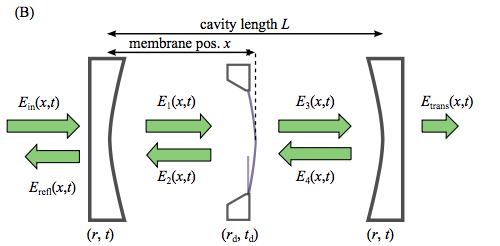
\includegraphics[scale=0.8]{transfer_matrix.png}
\caption{Two identical cavities: The left cavity shows how the membrane position $x$ is placed in the standing wave ``bubble" $2kx$ and the right cavity shows the schematic of the subcavity amplitude field analysis.}
\label{fig:transfer_model}
\end{figure}

The Fabry-Perot cavity is now divided into two sub-cavities of lengths $L_1$ and $L_2$, respectively (left and right sides) separated by a membrane with amplitude reflection coefficient $r_m$ and transmission $t_m$. We apply the same method as in section \ref{sec:cav_eom} and get a set of coupled equations

\begin{subequations}
\begin{align}
E_1 & = it_1E_{in} + r_1E_2e^{ikL_1} \\
E_2 & = r_mE_1e^{ikL_1} + it_mE_4e^{ikL_2} \\
E_3 & = it_mE_1e^{ikL_1} + r_mE_4e^{ikL_2} \\
E_4 & = r_2E_3e^{ikL_2} \\
E_{refl} & = it_1E_2e^{ikL_1} + r_1E_{in} \\
E_{trans} & = it_2E_3e^{ikL_2}
\end{align}
\end{subequations}
\noindent
We can obtain a solution for the variation in cavity resonance modulated by membrane position by writing up the closed system, i.e. excluding reflection and transmission, and find its eigenfrequencies

\begin{equation}
\begin{pmatrix}
E_{in} \\
E_{1} \\
E_{2} \\
E_{3} \\
E_{4}
\end{pmatrix}
  =
\begin{pmatrix}
1 & 0 & 0 & 0 & 0\\
it_1 & 0 & r_1e^{ikL_1} & 0 & 0 \\
0 & r_me^{ikL_1} & 0 & 0 & it_me^{ikL_2} \\
0 & it_me^{ikL_1} & 0 & 0 & r_me^{ikL_2} \\
0 & 0 & 0 & r_2e^{ikL_2} & 0 \\
r_1 & 0 & it_1e^{ikL_1} & 0 & 0 \\
0 & 0 & 0 & it_2e^{ikL_2} & 0
\end{pmatrix} 
\begin{pmatrix}
E_{in} \\
E_{1} \\
E_{2} \\
E_{3} \\
E_{4}
\end{pmatrix} \\
\label{eq:transfer_matrix}
\end{equation}
\noindent
As an approximation the mirrors will be assumed to yield high finesse $r_{1,2} \approx 1$, also we will neglect absorption of the membrane, i.e. the imaginary part of the index of refraction is set to zero; $\Im[n] = 0$. We will also assume that the membrane is placed in the middle such that the subcavity lenghts become equal, we rewrite the cavity length $L_1 \rightarrow L + x$ and $L_2 \rightarrow L - x$, where $x$ is the membrane position with respect to the end mirror. The approximated solution \cite{jayich2008} then becomes

\begin{equation}
\frac{\omega_c(x)}{FSR} = 2(\phi_m + \cos^{-1}(\left|r_m\right|\cos(2k\Delta x))),
\label{eq:resonance_var}
\end{equation}

where $\phi_m$ is the complex phase of the membrane refrection $r_m$. We plot equation \eqref{eq:resonance_var} by setting the membrane thickness unrealistically low $d = 0.01$ \SI{}{\nano\meter}, varying the reflection by changing the index of refraction $n$ and scanning the membrane through one wavelength for various reflectivties of the membrane. A half wavelength is defined as a standing wave ``bubble" in figure \ref{fig:transfer_model}.

\begin{figure}[H]
\centering
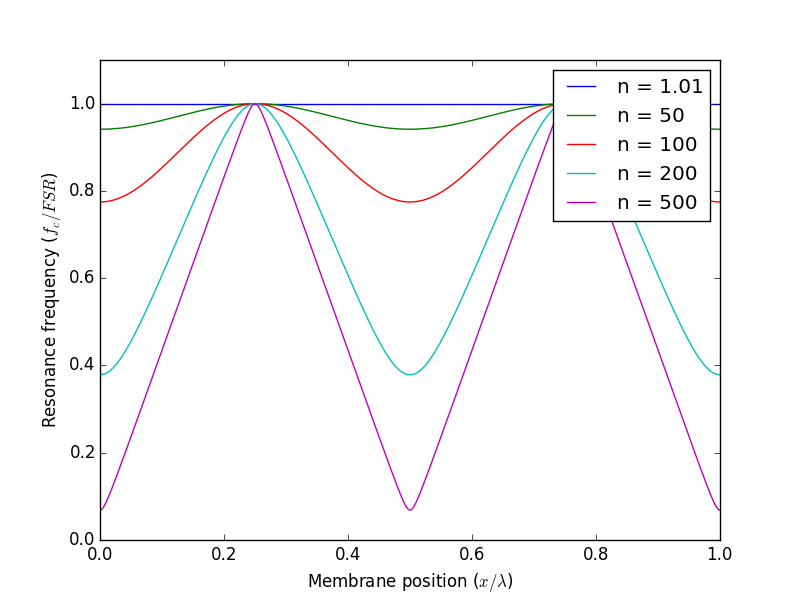
\includegraphics[scale=0.8]{transfer_matrix_python.png}
\caption{The membrane position is moved through one wavelength $\lambda$ with various reflection coefficients (index of refraction). The thickness is $d = 0.01$ \SI{}{\nano\meter} for the numerical simulation.}
\label{fig:transfer_model_plot}
\end{figure}

We previously introduced the optical frequency shift per displacement as $G = \frac{\partial\omega_c}{\partial x}$, i.e. the slope of the figure \ref{fig:transfer_model_plot}. It is an important parameter in our model, since our optically induced effects are quadratic in $G$. Clearly it must be advantageous to have the membrane placed at the steepest point on the slope. We also see that a membrane with fairly high reflectivity, gives a steeper slope and therefore also a higher coupling $G$. Another important message to take from this section is that the $FSR$ is no longer well defined.